\iffalse
\title{Assignments}
\author{Mokshith ee24btech11009}
\section{subjective}
\fi
%\begin{enumerate}
\item Six $X$'s have to be placed in the squares of figure below in such a way that each row contain at least one $X$. In how many different ways can this be done.
\hfill{(s1978)}\\
\begin{center}
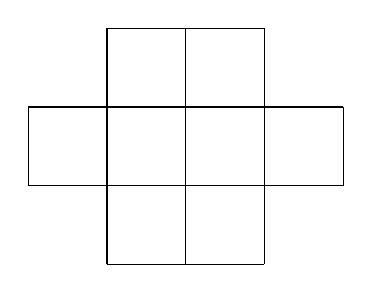
\begin{tikzpicture}
\draw (1,0) -- (3,0);
\draw (0,1) -- (4,1);
\draw (0,2) -- (4,2);
\draw (1,3) -- (3,3);
\draw (0,1) -- (0,2);
\draw (1,0) -- (1,3);
\draw (2,0) -- (2,3);
\draw (3,0) -- (3,3);
\draw (4,1) -- (4,2);
\end{tikzpicture}
\end{center}
%\end{enumerate}
